\section{Auswertung}
\subsection{a)}  %--> idk wie wir layout mache wollen/section gerüst usw
Zur Bestimmung der vorher definierten Zeitkonstante RC wird der Entladungsvorgung des Kondensators untersucht.
Dazu werden die gemessenen Spannungen $U_c$ bei entsprechender Zeit $t$ in einem halblogarithmischen Diagramm dargestellt.
Anschließend folgt die Annährung einer linearen Ausgleichsgerade durch Python, mit einem charakteristischen Steigungsparamter
der Form $1/RC$. Die Parmater der Gerade lauten.
% \begin{align*}
    % 1/{RC} &= 
    % b &= 
% \end{align*}
 
\begin{figure}
    \centering 
    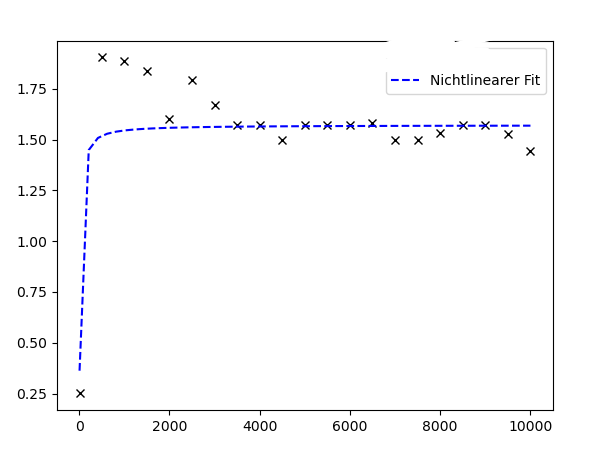
\includegraphics[width=\textwidth]{build/plot1.pdf}
    \caption{Messwerte der Entladungskurve in halblogarithmischer Darstellung mit Ausgleichsgerade}
    \label{plt:plot1}
\end{figure} 